%% This is file `jcomp-template.tex',
%% 
%% Copyright 2017 Elsevier Ltd
%% 
%% This file is part of the 'Elsarticle Bundle'.
%% ---------------------------------------------
%% 
%% It may be distributed under the conditions of the LaTeX Project Public
%% License, either version 1.2 of this license or (at your option) any
%% later version.  The latest version of this license is in
%%    http://www.latex-project.org/lppl.txt
%% and version 1.2 or later is part of all distributions of LaTeX
%% version 1999/12/01 or later.
%% 
%% The list of all files belonging to the 'Elsarticle Bundle' is
%% given in the file `manifest.txt'.
%% 
%% Template article for Elsevier's document class `elsarticle'
%% with harvard style bibliographic references
%%
%% $Id: jcomp-template.tex 100 2017-07-14 13:15:12Z rishi $
%%
%% Use the option review to obtain double line spacing
%\documentclass[times,review,preprint,authoryear]{elsarticle}

%% Use the options `twocolumn,final' to obtain the final layout
%% Use longtitle option to break abstract to multiple pages if overfull.
%% For Review pdf (With double line spacing)
\documentclass[times,twocolumn,final]{elsarticle}
%% For abstracts longer than one page.
%\documentclass[times,twocolumn,review,longtitle]{elsarticle}
%% For Review pdf without preprint line
%\documentclass[times,twocolumn,review,nopreprintline]{elsarticle}
%% Final pdf
%\documentclass[times,final]{elsarticle}
%%
%\documentclass[times,twocolumn,final,longtitle]{elsarticle}
%%


%% Stylefile to load JCOMP template
\usepackage{jcomp}
\usepackage{framed,multirow}
\usepackage{amsmath}
%% The amssymb package provides various useful mathematical symbols
\usepackage{amssymb}
\usepackage{latexsym}

% Following three lines are needed for this document.
% If you are not loading colors or url, then these are
% not required.
\usepackage{url}
\usepackage{xcolor}
\definecolor{newcolor}{rgb}{.8,.349,.1}

\journal{Computer Methods and Programs in Biomedicine}

\begin{document}

\verso{Anahita A. Seresti \textit{et al}}

\begin{frontmatter}

\title{Contrast Dispersion Title \tnoteref{tnote1}}%


\author[1]{Anahita \snm{A. Seresti}}

\author[2]{M. Owais \snm{Khan}\corref{cor1}}
\cortext[cor1]{Corresponding author: Department of Electrical, Computer and Biomedical Engineering, Toronto Metropolitan University, Toronto, 350 Victoria Street, Toronto, Ontario, M5B 2K3, Canada; Email: owaiskhan@torontomu.ca }


\address[1]{Department of Electrical, Computer and Biomedical Engineering, Toronto Metropolitan University, 350 Victoria Street, Toronto, M5B 0A1, Canada}


\received{1 May 2013}
\finalform{10 May 2013}
\accepted{13 May 2013}
\availableonline{15 May 2013}
%\communicated{S. Sarkar}


\begin{abstract}
%%%
\textbf{Background and Objectives}: Contrast Dispersion

\textbf{Methods}: Contrast Dispersion 

\textbf{Results}: Contrast Dispersion

\textbf{Conclusions}: Contrast Dispersion
%%%%
\end{abstract}


\begin{keyword}
% MSC codes here, in the form: \MSC code \sep code
% or \MSC[2008] code \sep code (2000 is the default)
% Keywords
\KWD Contrast Dispersion \sep Contrast Dispersion\sep Contrast Dispersion\sep Contrast Dispersion
\end{keyword}

\end{frontmatter}

%\linenumbers

%% main text

 %--------------------------------------- Introduction -----------------------------------------

\section{Introduction}
Contrast Dispersion
%--------------------------------------- METHODOLOGY -----------------------------------------
\section{Methods}

%------------- Problem Statement ----------------------
\subsection{Contrast Transport and Blood Flow}
The implementation of the TAFE method was discussed by detail in Eslami et al. [2015, 2022]. In short, two partial differential equations are the key components of implementation of this method: Navier-Stokes equations, simulating the blood flow assuming as a newtonian and incompressable fluid, and Advection-Diffusion equation, modeling the contrast agent transport in the blood. The governing equations of the Navier-Stokes equation is presented below:

\begin{equation}
\dfrac{\partial U}{\partial t} + (U. \nabla)U + \dfrac{\nabla P}{\rho} = \nu \nabla^2U,\quad \quad \quad \nabla.U=0
\end{equation}

Where $U$ is the time-dependant velocity vector field, $P$ is the pressure field inside the geometry domain, $\rho$ is the blood flow density, and $\nu$ is the dynamic viscosity. A neuman type boundary condition was assigned to the inlet of the vessel and a non-slip boundary condition ($u=0$) was assigned to the walls. The advection-diffusion equation is defined as below where $C(\frac{mg}{ml})$ is the contrast agent concentration: 

\begin{equation}
\dfrac{\partial C}{\partial t} + (U.\nabla )C = D\nabla ^2C
\end{equation}

Eslami et al [2022] in their work presented an equation for the quantitative flow rate estimate $Q_{TAFE}$ of the flow along the vessel. The equation was established based on assuming a unidirectional flow with minimal lateral flow distortion and the domainance advection in comparison to the diffusion. The method then suggest to use the cumulative volume at the axial locations down the vessel to find $Q_{TAFE}$. However, we used the same strategy to validate against the $v_{mean}$, the mean blood velocity along the centerline direction of the vessel.

\begin{equation}
v_{mean} = \dfrac{\frac{\partial C}{\partial t}}{-\frac{\partial C}{\partial x}}
\end{equation}

The numerator of the above fraction, $\frac{\partial C}{\partial t}$ is the temporal derivative of the time-attenuation curve (TAC) with the $\frac{HU}{s}$ unit, and $\frac{\partial C}{\partial x}$ can be found with takeng the derivative of the contrast at the centerline of the vessel with respect to the centerline direction with the unit of $\frac{HU}{cm}$.

%---------------- Simulations Setup ------------------------
\subsection{Simulations Setup}
\textit{CFD simulations} The direct numerical solution of the steady flow along a 3D non-axisymetric stenotic model were previously presented by M. Owais Khan et al. [2018]. Briefly, to characterize the turbulance transition in a stenosed artery we implemented the CFD simulations for Navier-Stokes equation on Oais flow solver [] for $Re=100-1000$. We used a second-order polynomial function for velocity and a first-order polynomial function for pressure. Figure 1 presents the axial and cross sectional view of the stenosed artery. The geometry was meshed in 6000 triangular elements. The simulation was run for 1 second with 10000 time steps. Figure ~\ref{Figure:Results_CFD} depicts the Q-criterion of the turbulance transition along the artery for $Re=100-1000$. 

\textit{Advection Diffusion Simulations} The advection diffusion equation was implemented using the FEniCs framework [] on the output of the CFD simulations. FEniCs is a library to implements PDEs based on the basis of the finite element methods on Python. To assign the inlet boundary conditions of the contrast agent we used the equation presented in Eslami et al. [2015]:

\begin{equation}
C_{inlet} =  C_{min} + 0.5 \times (C_{max}-C_{min}) \times [1-cos(\pi \times \dfrac{t-T_s}{T_d})]
\end{equation}

In this simulation $C_{min}$ and $C_{max}$ are the minimum and maximum of the concentration at the inlet. $T_s$ is the time that bolus arrives to the inlet, and $T_d$ is it takes for the bolus to arrive from the inlet to the outlet. In our simulations that we have a varying $Re$, we chose $T_d = 15-80s$. Fig 3 sheds more light on the contrast transition along the vessel.

\textit{Contrast Dispersion Simulations} The next step in our simulation to back-calculate the mean velocity according to waht presented in eq (3). In this simulation we fit a linear regression model to the time-attenuation curve at the inlet of the vessel, and the centerline-attenuation curve at the peak time of the advection diffusion output. The slope of the linear model fitted to each curves represents $\frac{\partial C}{\partial t}$ and $\frac{\partial C}{\partial x}$ respectively.


%FIGURE 0
\begin{figure*}[!t]
\centering
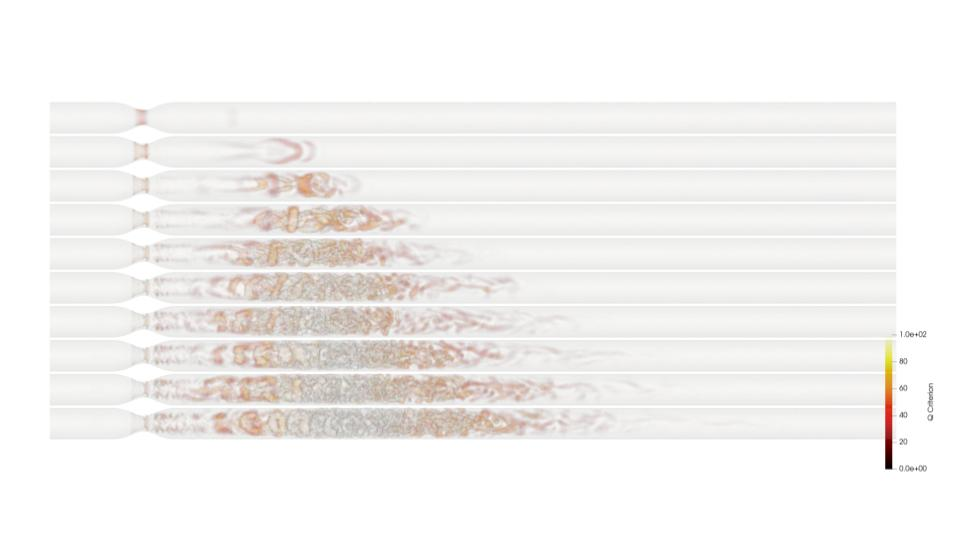
\includegraphics[width=0.8\textwidth]{./Figures/Figure2_Methods_CFD.jpg}
\caption{The results of implementing CFD simulations in stenosed pipe. changing $Re=100-1000$}
\label{fig:Results_CFD}
\end{figure*}


%------------------------------------ RESULTS ------------------------------------------------
\section{Results}
%1D Advection Diffusion Equation
\subsection{CFD Simulation Results}


%Figure 3
%\begin{figure*}[!t]
%\centering
%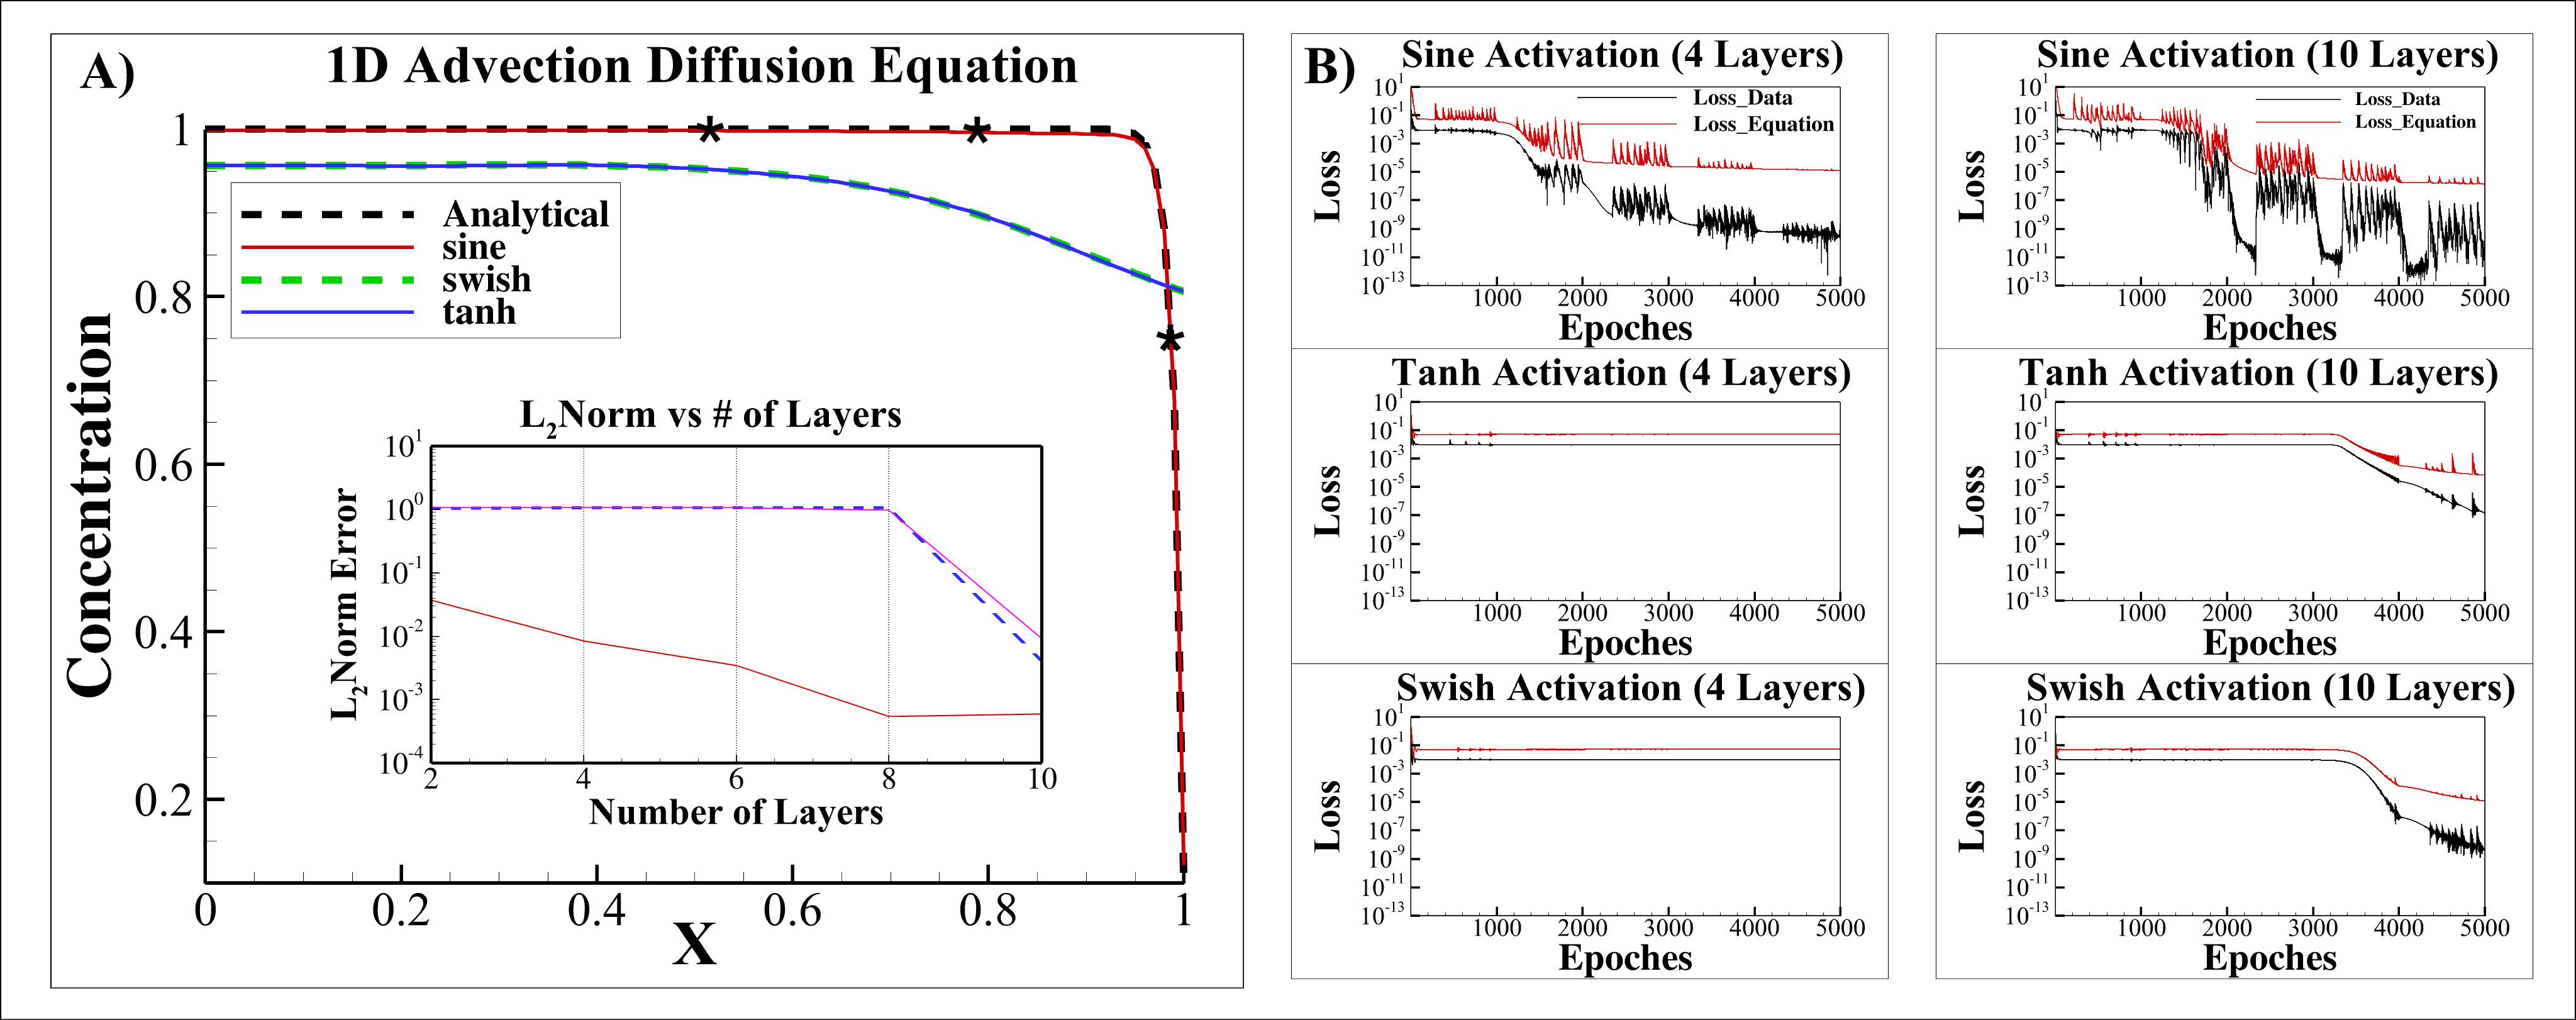
\includegraphics[width=0.95\textwidth]{./Figures/Figure3_AdvectionDiffusion}
%\caption{PINN solution for $sine$, $tanh$ and $swish$ activation functions for the 1D advection diffusion equation. A) Solution to the 1D advection-diffusion equation with the three activation functions using two neural network layers. Three sensor points were used (marked with *). The inset shows the changes in $L_{2}$-error norms with increasing number of layers. B) Mean squared errors for the three activation functions with 4 layers and 10 layers.}
%\label{Figure:Results_1}
%\end{figure*}

%2D Non-axisymmetric Stenosis
%\subsection{Test Case B: 2D Non-Axisymmetric Stenosis at Re=5000}
%Figure ~\ref{fig:Results_2}A show the cross-section velocity distribution for the $sine$, $tanh$ and $swish$ activation functions with increasing number of sensor points. The $sine$ activation function was able to capture the oscillations in the flow field even with only 200 sensor points, while at least 400 points were needed to reconstruct the oscillatory flow patterns in the post-stenotic regions for $tanh$ and $swish$ activation functions. These observations are also evident from the quantitative analysis in Figure ~\ref{fig:Results_2}C, which shows that $sine$ activation function was able to converge to an error of approximately 25\% with a sensor point density of only 16 (i.e., 400 sensor points), while both $tanh$ and $swish$ activation functions needed a sensor point density of approximately 40 (i.e, 1000 sensor point) to converge to the same error levels. In addition, only $sine$ activation function showed a monotonic reduction in errors while both $tanh$ and $swish$ activation functions demonstrated a non-monotonic reduction in errors. 



%Figure 4
%\begin{figure*}[!t]
%\centering
%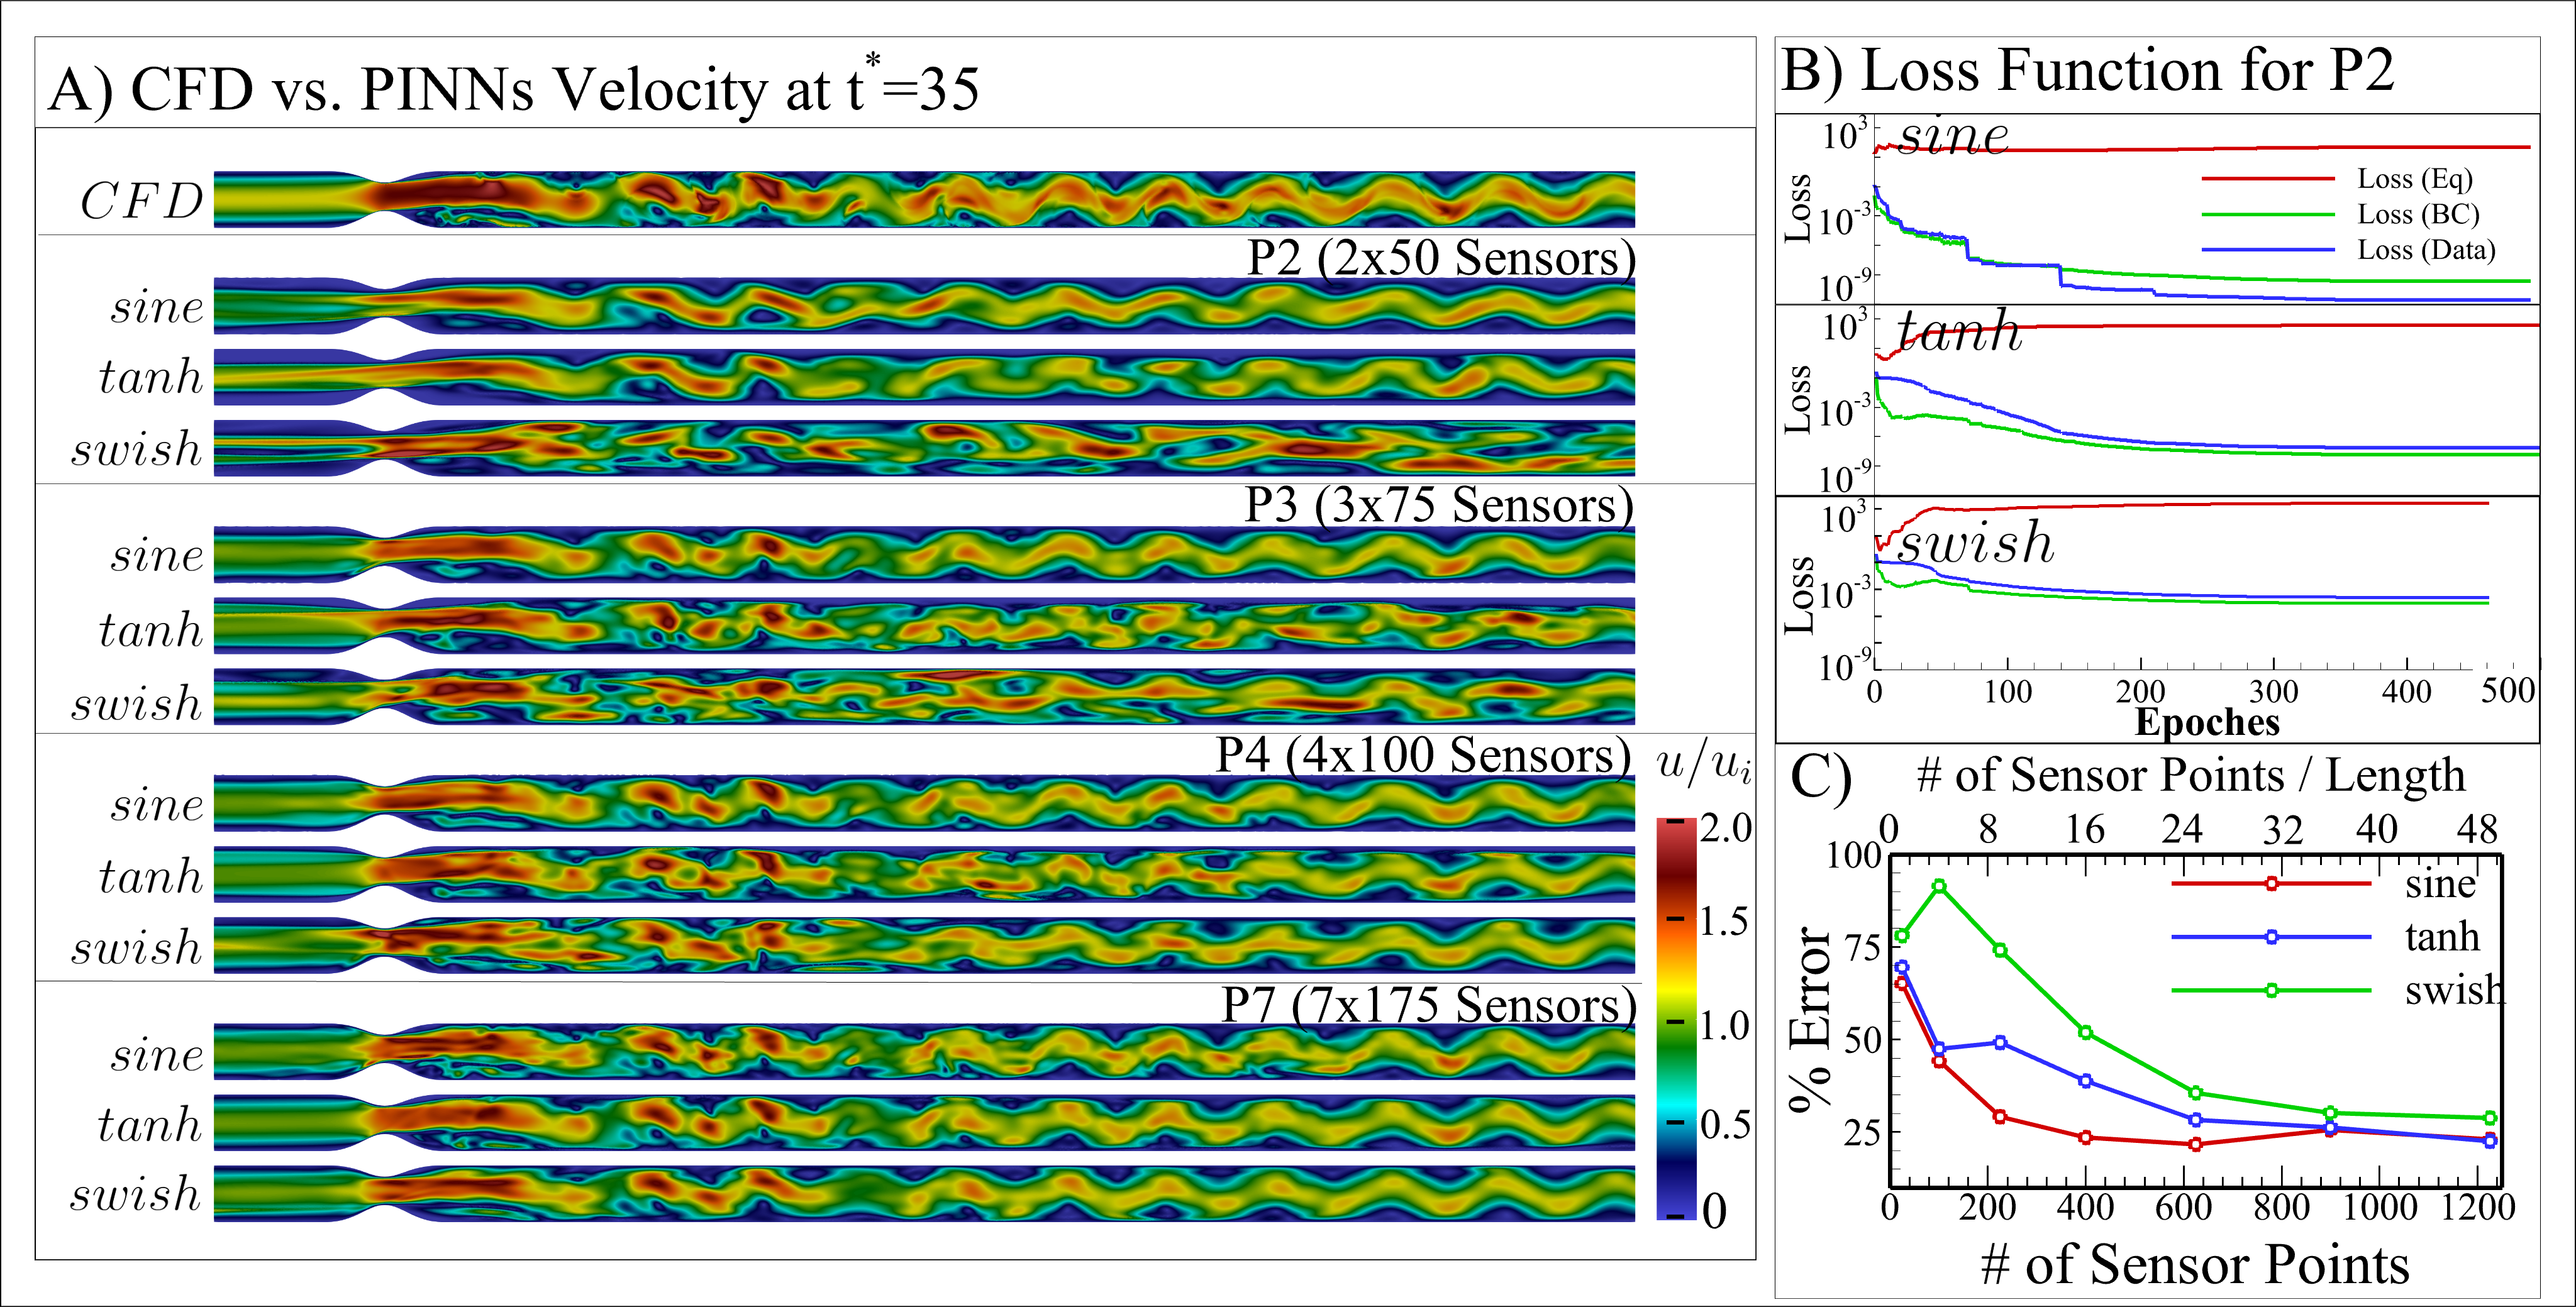
\includegraphics[width=0.95\textwidth]{./Figures/Figure4_StenosisResults_v2}
%\caption{PINNs solution for $sine$, $swish$ and $tanh$ activation functions for the 2D non-axisymmetric stenosis model at non-dimensional time of $t^{*}=35$ and Reynolds number of 5000. A) Reconstructed stream-wise velocity maps with increasing number of sensor points; B) Loss functions for P2 (i.e., with 2x5 sensors); C) Percent errors for the three activation functions with increasing sensor points and sensor point density.}
%\label{fig:Results_2}
%\end{figure*}


%3D Aortic Geometry
%\subsection{Test Case C: Patient-Specific 3D Aortic Geometry}
%Figure ~\ref{fig:Results_5} shows the performance of $sine$, $tanh$, and $swish$ activation functions in a 3D patient-specific aortic geometry at peak systole. Based on the qualitative velocity maps shown in Figure ~\ref{fig:Results_5}, it can be noted that a sensor point density of 40 (i.e, 800 sensor points) was needed to reconstruct the gross flow patterns observed in the ground-truth CFD simulations. The quantitative analysis, shown in Figure ~\ref{fig:Results_5}C, demonstrates that both $sine$ and $tanh$ had similar errors, while $swish$ had comparatively higher errors for the same number of sensor data points.

%POD analysis was performed to visualize the eigenspectra of the velocity field reconstructed from the three activation functions. Figure ~\ref{fig:Results_6} shows that for the case with 200 sensor points, all three activation functions showed similar Eigen spectra. However, with increasing number of sensor points, the $sine$ activation function was able to capture the energy content at higher modes much better than the other two activation functions, highlighting its ability to obtain high-frequency spatial structures in the velocity field . For example, for case with 800 sensor points and above, both $tanh$ and $swish$ activation functions were unable to adequately capture the kinetic energy in modes greater than 10. On the other hand, $sine$ activation function was able to better capture the energy content at these modes, matching well to the Eigen spectra obtained from the ground-truth CFD simulations. 

%Figure 5
%\begin{figure*}[!t]
%\centering
%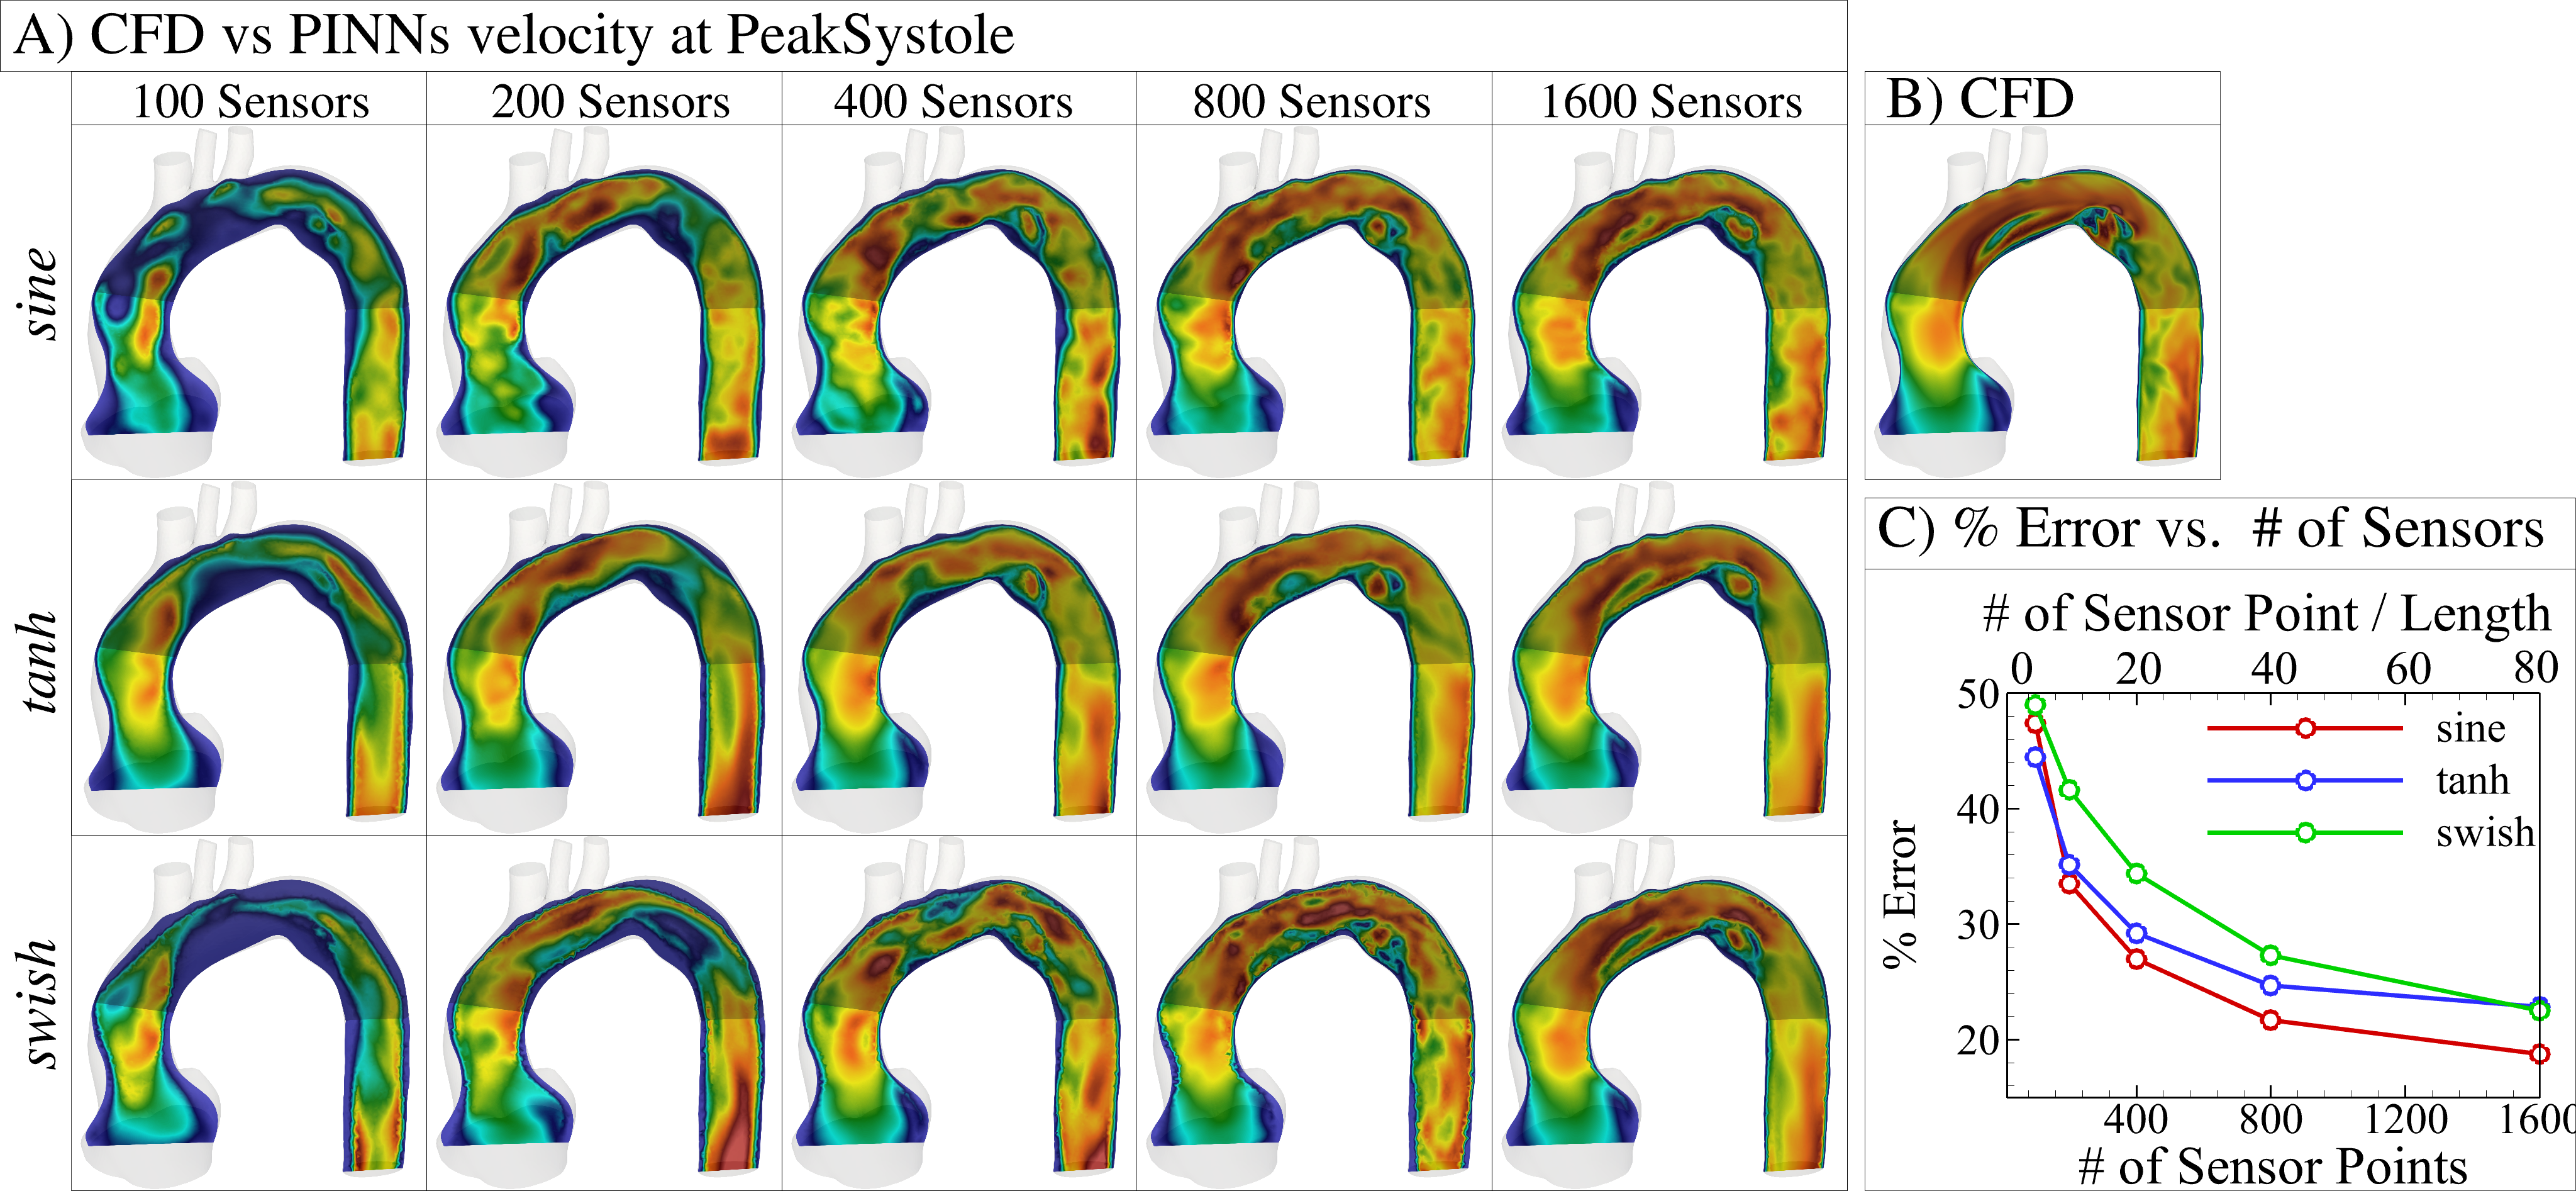
\includegraphics[width=0.95\textwidth]{./Figures/Figure5_Aorta}
%\caption{PINN solution for $sine$, $swish$ and $tanh$ activation functions for the 3D patient-specific aortic model at peak systole and Reynolds number of 823. A) PINNs-derived velocity maps with increasing number of sensor points from $100-1600$ at peak systole; B) Ground-truth solution obtained from CFD simulations; C)  Percent errors for the three activation functions with increasing sensor points and sensor point density. }
%\label{fig:Results_5}
%\end{figure*}

%Figure 6
%\begin{figure*}[!t]
%\centering
%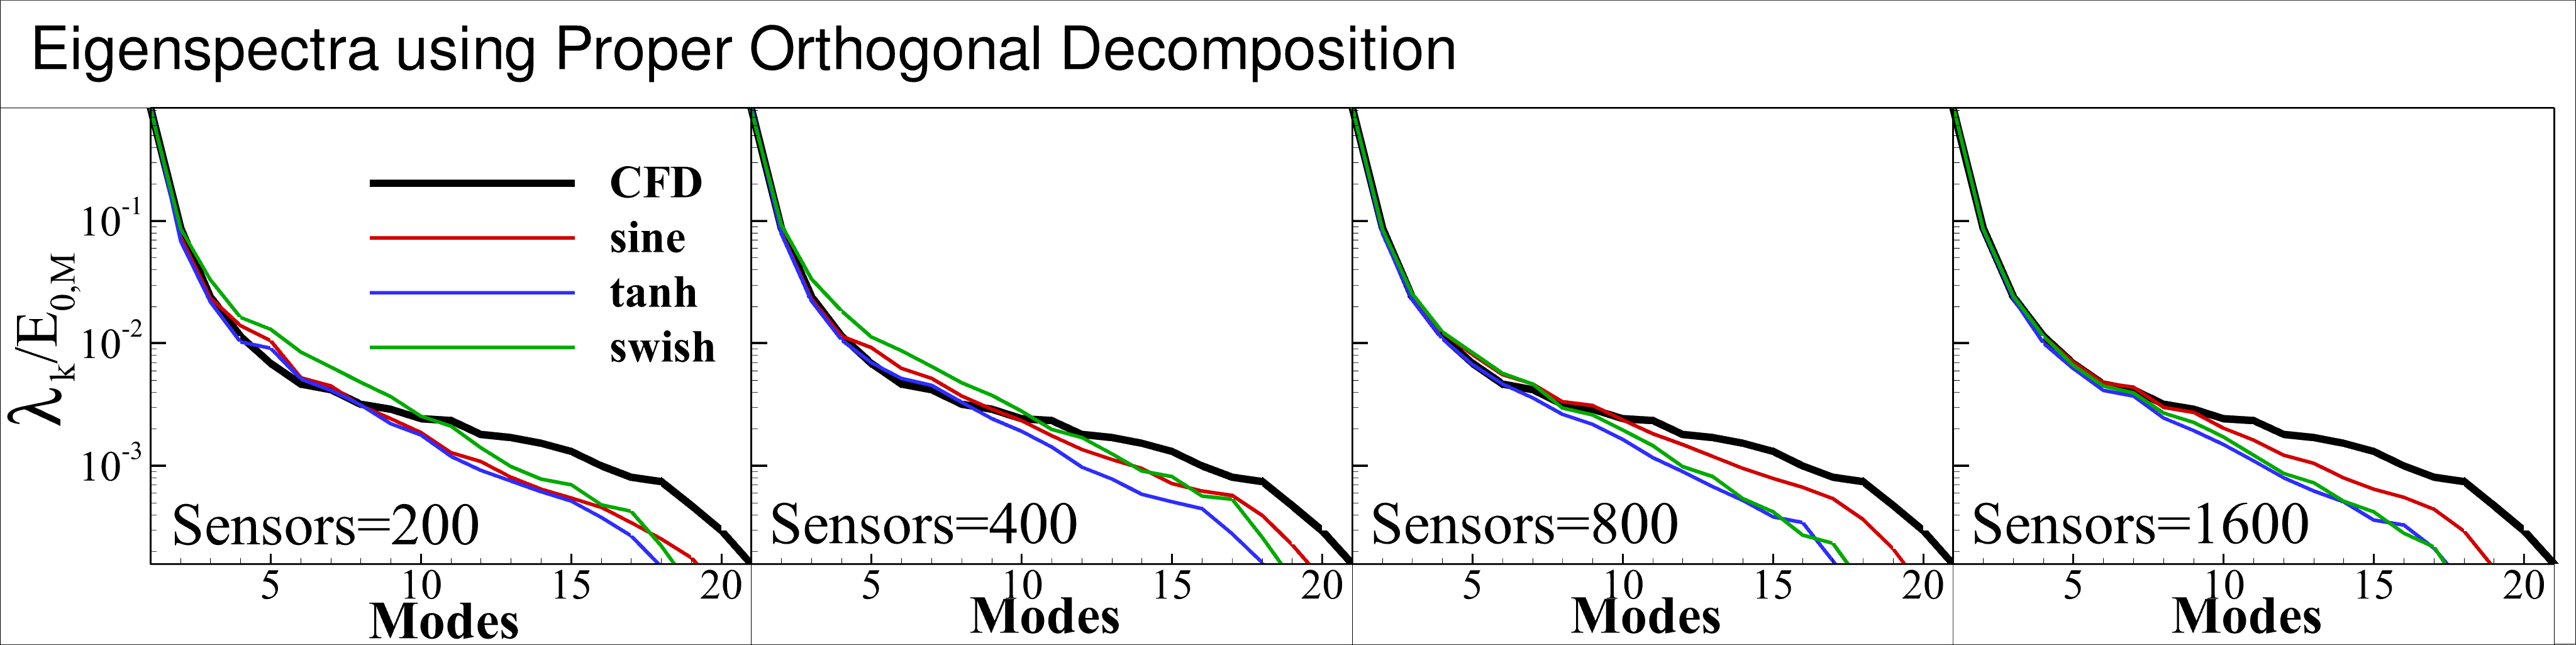
\includegraphics[width=0.95\textwidth]{./Figures/Figure6_Aorta_POD}
%\caption{Eigenspectra of temporal autocorrelation derived from proper orthogonal decomposition analysis for the 3D aorta model. Eigenvalue for each mode has been normalized by the sum of all eigenvalues from modes 0 to 20.}
%\label{fig:Results_6}
%\end{figure*}

%%%%%%%%%%%%%%%%% DISCUSSION %%%%%%%%%%%%%%%%%%%%
\section{Discussion}
%\subsection {Higher Performance of $sine$ Activation Function to Model Complex Cardiovascular Flows}
%Activation functions play a key role in the training process of the neural networks and determine the overall performance and accuracy of the learned solutions. Common activation functions, such as $ReLU$, $tanh$, $swish$, and $sigmod$, have been observed and proven to suffer from substantial inefficiency on learning high-frequency functions, even with increased network complexity \citep{Tancik2020_PINNs}. The failure of standard neural networks on high-frequency functions is a well-known phenomenon, called spectral bias \citep{Rahman2019_PINNs}. These limitations of standard activation functions can be problematic in modeling complex cardiovascular flows that often contain high-frequency spatio-temporal flow fluctuations. Indeed, recent evidences from super-resolution CFD simulations and experimental measurements have shown the presence and prevalence of high-frequency spatio-temporal flow fluctuations, often termed "turbulent-like" flows \citep{Khan2021_Aneurysms,Bruneau2023_Aneurysm} . These findings raise questions regarding the applicability of PINNs, specifically with conventional activation functions, to model complex, turbulent-like cardiovascular flows. 

%Our work builds on the recent developments in the field of computer vision, which have proposed remedies to learn high-frequency content with the use of Fourier features \citep{Tancik2020_PINNs} or $\omega_{0}$-scaled sine activation function \citep{Sitzmann2020_PINNs}. The former approach, which uses Fourier features, was introduced recently in the PINNs community by Wang et al. \citep{Wang2020_PINNs} but with the requirement to tune length scales of the Fourier features for each application. However, problem-specific tuning of length-scales is infeasible for cardiovascular applications, where flow conditions and geometric complexity can vary substantially depending on the anatomic location (e.g, aorta vs. cerebral vasculature) or flow conditions (e.g., aneurysm vs. stenosis). Hence, in our study, we have used the approach of Sitzmann et al., since their implementation is less sensitive to the choices of hyper-parameters of the neural network compared to the original Fourier feature approach. 

%A recent study by Moser et al. compared the performance of various neural network architecture for cardiovascular flow applications \citep{Moser2023_PINNs}. Interestingly, those authors demonstrated that the modified Fourier Network architecture, as proposed by Wang et al., had the poorest accuracy amongst all architectures considered. While the reason for these negative findings are unclear, it is possible that the length scales were not tuned adequately for the problem. Instead of modifying the neural network architecture, we have used $sine$ as an activation function in the hidden layers, following the implementation of Sitzmann et al.\citep{Sitzmann2020_PINNs}, and have shown that this approach resulted in substantially higher accuracy compared to other conventional activation functions.

%\subsection {Requirements on the Number of Sensor Points for Vascular Territories}
%One of the key strengths of PINNs is the ability to include known sensor data, such as those measured invasively in a patient or through imaging (e.g., 4D Flow MRI), into the loss function. These inclusion of sensor data can improve the accuracy of the learned solution, especially when no boundary condition information is supplied. For example, a recent study demonstrated that when using a purely physics-based neural network, the learned solutions were in closer agreement for idealized geometries (i.e., cylinder and bifurcations) compared to patient-specific geometries, such as cerebral aneurysms \citep{Moser2023_PINNs}. These observations highlight the need to include known sensor data into the neural network loss function to regularize the solution; however, there is no consensus on how many sensor points are needed to obtain converged solutions for cardiovascular flow applications.

%Our study is the first to establish the requirements on the number of sensor points needed for cardiovascular flow applications. Our findings demonstrate that at least 80 sensor points per $L/D$ are needed to obtain learned velocity fields with approximate errors of 20\%. These requirements were lower for 2D non-axisymmetric stenosis model where no reduction in errors were observed after 36 sensor points per $L/D$ for $tanh$ and $swish$ activation functions, and only 16 sensor points per $L/D$ for $sine$ activation functions. 

%Previous study by Arzani et al. have used approximately 125 sensor points when modeling an idealized 3D cerebral aneurysm at Reynolds of 320 using the $swish$ activation function \citep{Arzani2021_PINNs}. Although our neural network architecture was similar to theirs, we used a patient-specific aortic geometry at much higher Reynolds number of 823,  resulting in more complex flow conditions. While it is challenging to compare the sensor point density between our studies since the anatomies are vastly different, using the aneurysm dimensions from their paper (L=0.8, aneurysm size and D=0.8, aneurysm neck), we can estimate their sensor point density as 125 points per $L/D$. This density is much higher than our proposed threshold of 80 sensor points per $L/D$, and thus, their learned velocity was likely converged. 

%\subsection {Convergence Properties with Increasing Sensor Points}
%One key observation from our study is that, regardless of the activation function used, the errors tended to asymptote around 20 to 25\%. For example, in the 2D non-axisymmetric stenosis model, the errors tended to stagnate at 25\% even with a 2 or 4 fold increase in the number of sensor points. Similarly, in the 3D patient-specific aortic model, the errors tended to stagnate at 20-25\%. These findings highlight the inherent and known limitations of neural networks related convergences of higher frequency data. Previous studies have demonstrated that neural networks tend to initially fit to data of lower complex, but require substantially higher iterations to converge to high frequency data. These previous findings are in line with our observations that with increasing sensor points, the errors tended to stagnate around 20 - 25\% and would have required substantially higher training data to reduce those errors.

%Another interesting observation relates to the monotonic convergence property of the $sine$ activation function. We have demonstrated that as the sensor point density increased, $sine$ activation function was able to converge much faster and with a monotonic reduction in errors compared to the $tanh$ and $swish$ activation functions. For example, in the case of the 2D non-axisymmetric stenosis model, which had high spatial frequencies, both $tan$ and $swish$ activation functions had non-monotonic decrease in errors whereas $sine$ activation function demonstrated a monotonic decrease. In contrast, for the 3D patient-specific aorta, all three activation functions produced a monotonic decrease in error, likely because the flow field in the 3D aortic geometry lacked complex and dynamical flow structures (e.g., high spatial frequencies, oscillations) compared to those obtained in the 2D non-axisymmetric stenosis model at the Reynolds number of 5000.

%\subsection{Implications for Cardiovascular Flow Modeling}
%These findings have important implications for modeling cardiovascular flows. One of the key applications of PINNs in cardiovascular flows is to integrate imaging measurements with physics to improve the overall accuracy of the learned solution. For example, 4D Flow MRI is  being used increasingly in the clinic to non-invasively obtain velocity field in patients, but suffers from poor spatial resolutions, typically on the order of 0.1 cm. In the case of a healthy aorta, this would translate to approximately 700 points (i.e., D=3cm and L=10cm) using a conventional 4D Flow MRI sequence. Based on our findings, we would require a sensor point density of at least 80, which translates to approximately 266 sensor points for a similarly-sized aorta. Hence, there is an exciting opportunity to substantially improve the accuracy of velocity measurements from existing 4D Flow MRI sequence by integrating PINNs into them. 

%Another key implication relates to modeling "turbulent-like" blood flows, such as those observed under pathological conditions (e.g., stenosis, aneurysms). Our findings demonstrate that $sine$-based activation function may have higher performance, especially in capturing complex dynamics, compared to conventional activation functions. For example, in our 3D patient-specific aortic example, $sine$-based activation function not only produced lower absolute errors but was also able to better capture the kinetic energy and Eigen spectra at higher modes. These differences could become more apparent under complex, quasi-turbulent flow conditions with high spatial frequencies (e.g., downstream of a narrow stenosis).


\section{Conclusions}
%We have tested the performance of a Fourier-based activation function with specialized initialization, against conventional activation functions for cardiovascular blood flow applications. Our findings can be summarized in three key points:

%\begin{itemize}
%\item $sine$ activation function has desirable properties (e.g., monotonic convergence) and better performance (e.g., lower errors) compared to traditional activation functions.
%\item sensor point density of at least 80 per normalized length (i.e. L/D) is required to obtain sufficiently converged velocity field.
%\item absolute errors tend to stagnate around 20-25\% for patient-specific cardiovascular flows even with two- or four-fold increase in the number of sensor point density.
%\end{itemize}

\section*{Acknowledgements}
MOK would like to acknowledge funding from the Natural Science and Engineering Research Council of Canada. 

%%Vancouver style references.
\bibliographystyle{model1-num-names}
\bibliography{refs}


\end{document}

%%
